
\documentclass[${FONT}pt $DRAFT]{$DOCUMENT} % ,draft

%%
%% Capture ENV vars from envsubst
%%

\def\AFIVE{$AFIVE}
\def\COMMITHASH{$COMMIT_HASH}
\def\COMMITTS{$COMMIT_TS}
\def\COVER{$COVER}
\def\DOMAIN{$DOMAIN}
\def\EBOOK{$EBOOK}
\def\EMAIL{$EMAIL}
\def\KINDLE{$KINDLE}
\def\LARGE{$LARGE}
\def\NARROW{$NARROW}
\def\PHONE{$PHONE}
\def\PRINT{$PRINT}
\def\QR{$QR}
\def\RIDERO{$RIDERO}
\def\DMK{$DMK}
\def\TABLET{$TABLET}

%%
%% Constants
%%

\def\NIL{}
\def\TRUE{true}

%%
%% if selectors
%%


%% http://handyfloss.net/2007.08/latex-programming-how-to-implement-conditionals/

%% QR

\newif\ifqr

\ifx\QR\TRUE
  \qrtrue
\else
  \qrfalse
\fi

%% NARROW

\newif\ifnarrow

\ifx\NARROW\TRUE
  \narrowtrue
\else
  \narrowfalse
\fi

%% KINDLE

\newif\ifkindle

\ifx\KINDLE\TRUE
  \kindletrue
\else
  \kindlefalse
\fi

%% TABLET

\newif\iftablet

\ifx\TABLET\TRUE
  \tablettrue
\else
  \tabletfalse
\fi


%% PHONE

\newif\ifphone

\ifx\PHONE\TRUE
  \phonetrue
\else
  \phonefalse
\fi

%% DMK

\newif\ifdmk

\ifx\DMK\TRUE
  \dmktrue
\else
  \dmkfalse
\fi

%% PRINT

\newif\ifprint

\ifx\PRINT\TRUE
  \printtrue
\else
  \printfalse
\fi

%% EBOOK

\newif\ifebook

\ifx\EBOOK\TRUE
  \ebooktrue
\else
  \ebookfalse
\fi

%% LARGE

\newif\iflarge

\ifx\LARGE\TRUE
  \largetrue
\else
  \largefalse
\fi

%% DMK

\newif\ifdmk

\ifx\DMK\TRUE
  \dmktrue
\else
  \dmkfalse
\fi

%% TITLE

\newif\iftitle

\ifx\TITLE\TRUE
  \titletrue
\else
  \titlefalse
\fi


% globals
\newlength{\marginparoffset}
\setlength{\marginparoffset}{0mm}


\usepackage[T2A]{fontenc}
\usepackage{tikz}
\usepackage{tocloft}
\usepackage{geometry}
\usepackage[utf8]{inputenc}
\usepackage[english,russian]{babel}


%% hyphenation in tt
\usepackage[shortcuts]{extdash}

% for proper ' and `
\usepackage{textcomp}
\usepackage{upquote}

% to replace strings
\usepackage{xstring}

% extra space at the end of macros
\usepackage{xspace}

% linebreaks in verbatim for mobile
\usepackage{spverbatim}

% http://www.khirevich.com/latex/microtype/
\usepackage[
  activate={true, nocompatibility},
  final,
  tracking=true,
  kerning=true,
  spacing=true,
  factor=1100,
  stretch=10,
  shrink=10
]{microtype}

% better captions
\usepackage[font=small]{caption}

\captionsetup{labelsep=period}

\captionsetup[listing]{name=Листинг}
\captionsetup[figure]{name=Рис.}

% https://tex.stackexchange.com/a/417276
% ifthispageodd macro
\usepackage{scrextend}

% underline
\usepackage[normalem]{ulem}

% for QR codes in
\usepackage{qrcode}

% to have bold tt fonts in code listings
\usepackage{bold-extra}

% better macro args
\usepackage{xparse}

% file trees
\usepackage{dirtree}

%% defaults

%% offset = 0.2em
%% width = 1em
%% sep = 0.2em
%% rule-width = 0.4pt
%% dot-size = 1.6pt

% \setlength{\DTbaselineskip}{1.2em}

\DTsetlength{0.2em}{1em}{0.2em}{0.4pt}{0pt}


% code highlight
\usepackage[newfloat=true]{minted}
\usemintedstyle{print}
%% \setminted{fontsize=\small} %% reduce minted font
\SetupFloatingEnvironment{listing}{placement=H}

\ifnarrow
\setminted{breaklines=true}
\fi

% mobile headers
\ifnarrow
\usepackage{sectsty}
\sectionfont{\raggedright}
\subsectionfont{\raggedright}
\subsubsectionfont{\raggedright}
\fi

% index
\usepackage{index}
\newindex{default}{idx}{ind}{Предметный указатель}
\usepackage[
  unbalanced,
  itemlayout=abshang,
  indentunit=0.25em,
  totoc
]{idxlayout}
\ifnarrow
\idxlayout{columns=1}
\else
\idxlayout{columns=2}
\fi

\usepackage{setspace}


% href ursl for ebooks
\ifebook
\usepackage[hidelinks, hyperindex=false]{hyperref}
\fi


% no indent for items in lists (in mobile)
\ifnarrow
\usepackage{enumitem}
\setlist[itemize]{leftmargin=*}
\fi

%% geometry presets
\input{$GEOMETRY}

%% \geometry{showframe} %% debug frames

\setlength{\parskip}{0.32em}

\pagestyle{plain}
\pagenumbering{arabic}

\setcounter{tocdepth}{1}

\widowpenalty=10000
\clubpenalty=10000
\tolerance=500
\hyphenpenalty=500
\hfuzz=0.5pt
\emergencystretch=5pt


\usetikzlibrary{shapes.geometric, arrows, positioning, decorations.markings}

\ifnarrow
\tikzstyle{entity} = [rectangle, inner sep=3mm, minimum width=2.7cm, text centered, draw=black]
\else
\tikzstyle{entity} = [rectangle, inner sep=3mm, minimum width=3.0cm, text centered, draw=black]
\fi

\tikzstyle{arrow} = [thick,->,>=stealth,line width=0.4pt]

\tikzstyle{arrowHuge} = [thick, decoration={markings,mark=at position
   1 with {\arrow[semithick]{open triangle 60}}},
   double distance=1.4pt, shorten >= 5.5pt,
   preaction = {decorate},
   postaction = {draw,line width=1.4pt, white,shorten >= 4.5pt}]


\def\Plus{\texttt{+}}
\def\Minus{\texttt{-}}

\def\linegap{\vspace{1.25em}}

\def\arr{$\to$\xspace}

\def\enter{\textbf{Enter}}

\def\tilde{\raisebox{-1mm}{\textasciitilde{}}}

\newcommand{\slurp}{\vspace{-1em}}

\newcommand{\coderef}[1]{(строка~#1)\xspace}

\newcommand{\coderefs}[1]{(строки~#1)\xspace}

\newenvironment{teaser}{\vspace{-3em}\slshape}{\vspace{1em}}

\newcommand{\eng}[1]{(англ.~#1)}

\newcommand{\RNum}[1]{\uppercase\expandafter{\romannumeral #1\relax}}

% https://tex.stackexchange.com/questions/44361/
\DeclareTextFontCommand{\code}{\ttfamily\hyphenchar\font=45\relax}

\ifprint
\newcommand{\page}[1]{(с.~\pageref{#1})}
\newcommand{\fig}[1]{(рис.~\ref{#1})}
\newcommand{\lis}[1]{\xspace(листинг~\ref{#1})}
\fi

\ifebook
\newcommand{\page}[1]{\hyperref[#1]{\uline{(с.~\pageref{#1})}}}
\newcommand{\fig}[1]{\hyperref[#1]{\uline{(рис.~\ref{#1})}}}
\newcommand{\lis}[1]{\hyperref[#1]{\uline{(листинг~\ref{#1})}}}
\fi

\ifnarrow
\newcommand{\chart}[1]{\begin{center}\input{#1}\end{center}}
\else
\newcommand{\chart}[1]{\input{#1}}
\fi

\NewDocumentCommand{\pagebreaklarge}{O{4}}{\iflarge\pagebreak[#1]\fi}

\newcommand{\noindentnarrow}{\ifnarrow\noindent\fi}

\def\splitter{{\noindent\centering\rule{3cm}{.4pt}\par}}

\def\blank{\clearpage{\pagestyle{empty}\cleardoublepage}}

%% #1 text
%% #2 URL
%% #3 QR label
%% #4 offset
\ifprint
\NewDocumentCommand{\footurl}{ m m O{} o }{%
#1%
\footnote{\raggedright\StrSubstitute{#2}{https://}{}\ifdmk\hspace{0.1em}\tiny{.}\fi}%
\marginpar{%
\IfNoValueTF{#4}{}{\vspace{#4}}%
\vspace{-5.5mm}%
\ifthispageodd{\raggedright}{\raggedleft}%
\ifqr\qrcode[height=10mm]{#2}\else\begin{tikzpicture}
\draw (0,0) -- (1,0) -- (1,1) -- (0,1) -- (0,0);
\end{tikzpicture}
\fi%
\\\vspace{1mm}\tiny{#3}\vspace{12mm}}%
}%
\fi

\ifebook
\NewDocumentCommand{\footurl}{ m m O{} O{} }{\href{#2}{\uline{#1}}}
\fi

\newcommand{\smartlink}[2]{%
\ifprint
\texttt{#1}%
\fi
\ifebook
\href{#2}{\uline{#1}}%
\fi
}

\def\EMAILLINK{\smartlink{\EMAIL}{mailto:\EMAIL}}

\def\SITELINK{\smartlink{\DOMAIN}{https://\DOMAIN}}

%% small non-breaking space
%% https://tex.stackexchange.com/questions/76132/
\newcommand{\tuple}[1]{\textlangle\,#1\,\textrangle}

\newminted[clojure]{clojure}{}

\ifprint
\def\codeindent{0mm}
\fi

\ifebook
\def\codeindent{\parindent}
\fi

\newminted[clojure/lines]{clojure}{linenos, xleftmargin=\codeindent}

\newminted[xml/lines]{xml}{linenos, xleftmargin=\codeindent}

\newminted[text/lines]{text}{linenos, xleftmargin=\codeindent}

\newminted[python/lines]{python}{linenos, xleftmargin=\codeindent}

\newminted[json/lines]{json}{linenos, xleftmargin=\codeindent}

\newminted[sql/lines]{sql}{linenos, xleftmargin=\codeindent}

\newminted[yaml/lines]{yaml}{linenos, xleftmargin=\codeindent}

\newminted[json]{json}{}

\newminted[lisp]{lisp}{}

\newminted[yaml]{yaml}{}

\newminted[bash]{console}{}

\newminted[bash/lines]{bash}{linenos, xleftmargin=\codeindent}

\newminted[python]{python}{}

\newminted[htmldjango]{htmldjango}{}

\newminted[js]{js}{}

\newminted[java]{java}{}

\newminted[javascript]{javascript}{}

\newminted[php]{php}{}

\newminted[xml]{xml}{}

\newminted[diff]{diff}{}

\newminted[sql]{sql}{}

\newminted[http]{http}{}

\newminted[text]{text}{}

\newminted[ini]{ini}{}

\newenvironment{english}{\begin{otherlanguage}{english}}{\end{otherlanguage}}


\author{Иван Гришаев}
\title{Clojure на производстве. Том второй}
\date{}

\usepackage{pdfpages}

%%
%% Kindle or Phone
%%
\ifnarrow

%% Remove labels for subchapters
\usepackage{titlesec}
\titlelabel{}

%% Small page numbers
\usepackage{fancyhdr}
\fancypagestyle{plain}{
  \fancyhf{}
  \fancyfoot[C]{\tiny\thepage}}
\pagestyle{plain}

\fi

%% add space b/w number and footnote
\let\oldfootnote\footnote
\renewcommand\footnote[1]{\oldfootnote{\hspace{1mm}#1}}


%% for ebook, remove top margin for ToC
\ifebook
\setlength{\cftbeforetoctitleskip}{0pt}
\setlength{\cftaftertoctitleskip}{2em}
\fi

\begin{document}


\hyphenation{In-te-rac-ti-on}
\hyphenation{пред-шес-т-вен-ни-ка}
\hyphenation{пре-ды-ду-ще-го}
\hyphenation{Cre-a-te}
\hyphenation{Re-ad}
\hyphenation{Up-da-te}
\hyphenation{De-le-te}
\hyphenation{Java-Script}
\hyphenation{Chro-me}
\hyphenation{clo-ju-re}
\hyphenation{Clo-ju-re-Script}
\hyphenation{Cof-fee-Script}
\hyphenation{com-po-ju-re}
\hyphenation{com-po-nent}
\hyphenation{do-cu-men-ta-ti-on}
\hyphenation{au-to-comp-le-te}
\hyphenation{асинх-рон-ны-ми}
\hyphenation{брау-зер}
\hyphenation{вер-ну-ла}
\hyphenation{возвра-щает}
\hyphenation{возмож-нос-ти}
\hyphenation{дос-ту-па}
\hyphenation{дос-ту-пом}
\hyphenation{зави-си-мос-ти}
\hyphenation{зак-ры-ва-ет}
\hyphenation{зап-ро-са}
\hyphenation{зап-рос}
\hyphenation{ис-клю-че-ние}
\hyphenation{клиен-том}
\hyphenation{Фун-к-ц-ии}
\hyphenation{конф-ликт}
\hyphenation{крип-то-гра-фия}
\hyphenation{мно-жест-вен-ны-ми}
\hyphenation{наст-рой-ки}
\hyphenation{нейт-раль-ное}
\hyphenation{непус-тую}
\hyphenation{парал-лельно}
\hyphenation{пере-мен-ных}
\hyphenation{по-мес-тим}
\hyphenation{пов-тор}
\hyphenation{под-мно-жест-во}
\hyphenation{пос-ле}
\hyphenation{прик-лад-ных}
\hyphenation{проб-ле-му}
\hyphenation{проб-ле-мы}
\hyphenation{прог-рам-мис-тов}
\hyphenation{проек-та-ми}
\hyphenation{произ-водст-ва}
\hyphenation{проис-хо-дит}
\hyphenation{прост-ран-ство}
\hyphenation{разно-образ-ны}
\hyphenation{разоб-рать}
\hyphenation{реак-ци-ей}
\hyphenation{рес-то-ра-нов}
\hyphenation{свой-ства}
\hyphenation{сис-те-ма}
\hyphenation{сис-те-ме}
\hyphenation{систе-мах}
\hyphenation{систе-мы}
\hyphenation{следую-щий}
\hyphenation{соз-дай-те}
\hyphenation{соз-дать}
\hyphenation{сос-лать-ся}
\hyphenation{сос-то-ит}
\hyphenation{сос-тоя-ние}
\hyphenation{сох-ра-ни-ли}
\hyphenation{тес-тах}
\hyphenation{тес-тов}
\hyphenation{триг-рам-мный}
\hyphenation{удоб-ства}
\hyphenation{упрос-тит}
\hyphenation{фак-ти-чес-кое}
\hyphenation{цент-ра-ли-зо-ван}
\hyphenation{час-тя-ми}
\hyphenation{эко-сис-те-му}
\hyphenation{Throw-ab-le}
\hyphenation{middle-wa-re}
\hyphenation{ме-та-дан-ны-ми}
\hyphenation{con-text}
\hyphenation{проч-тут}
\hyphenation{Out-Of-Me-mo-ry-Er-ror}
\hyphenation{File-Not-Found-Excep-tion}
\hyphenation{Arithmetic-Exception}
\hyphenation{Null-Pointer-Exception}
\hyphenation{Il-legal-Argu-ment-Excep-tion}
\hyphenation{Byte-Array-Input-Stream}
\hyphenation{Excep-tion-Info}
\hyphenation{мес-тах}
\hyphenation{дейс-твие}
\hyphenation{замк-ну-та}
\hyphenation{vo-la-ti-le}
\hyphenation{пер-сис-тент-ны-ми}
\hyphenation{тес-ти-ро-ва-нии}
\hyphenation{наз-ва-ния}
\hyphenation{пос-то-ян-ных}
\hyphenation{до-пус-тить}
\hyphenation{не-до-пус-ти-мо}
\hyphenation{всег-да}
\hyphenation{тес-ты}
\hyphenation{прос-тей-ший}
\hyphenation{мес-та}
\hyphenation{интег-ра-ци-он-ное}
\hyphenation{Se-le-ni-um}
\hyphenation{File-Not-Found-Excep-tion}
\hyphenation{Сле-ду-ю-щий}
\hyphenation{не-сколь-ко}
\hyphenation{не-удач}
\hyphenation{не-ко-то-рые}
\hyphenation{прог-рам-ми-ро-ва-нии}
\hyphenation{раз-ны-ми}
\hyphenation{Ma-ni-fold}
\hyphenation{уст-рой-ст-вом}
\hyphenation{воз-вра-ща-ет}
\hyphenation{con-fig}
\hyphenation{PG-DA-TA-BA-SE}
\hyphenation{mo-unt}
\hyphenation{com-po-nent}
\hyphenation{Hi-ka-ri-CP}
\hyphenation{ме-то-дах}
\hyphenation{DE-LE-TE}
\hyphenation{chro-me-dri-ver}
\hyphenation{ge-cko-dri-ver}
\hyphenation{при-ло-же-ние}
\hyphenation{Unix-Port}
\hyphenation{Net-Port}
\hyphenation{trans-form}
\hyphenation{wat-cher}
\hyphenation{per-sis-tent}
\hyphenation{In-teg-rant}
\hyphenation{de-scrip-ti-on}
\hyphenation{name-spa-ces}
\hyphenation{get-ting}
\hyphenation{за-пус-ка-ет}
\hyphenation{Re-fe-ren-ce}
\hyphenation{Gui-des}
\hyphenation{Get-ting}
\hyphenation{Star-ted}
\hyphenation{лис-тин-ге}
\hyphenation{fix-tu-res}
\hyphenation{res-pon-se}
\hyphenation{Con-tent}
\hyphenation{Ty-pe}
\hyphenation{app-li-ca-ti-on}
\hyphenation{oc-tet}
\hyphenation{stre-am}
\hyphenation{pa-rams}
\hyphenation{me-ta-da-ta}
\hyphenation{da-ta-sour-ce}
\hyphenation{some-thing}
\hyphenation{re-defs}
\hyphenation{lo-ca-le}
\hyphenation{glo-bal}
\hyphenation{le-vel}
\hyphenation{Cont-rol-ler}
\hyphenation{init-db}
\hyphenation{mid-dle-wa-re}
\hyphenation{не-дос-тат-ки}
\hyphenation{ло-ка-ция}
\hyphenation{COM-MIT-TED}
\hyphenation{git-ig-no-re}
\hyphenation{если}
\hyphenation{свойстве}
\hyphenation{свойство}
\hyphenation{судя}
\hyphenation{англ}
\hyphenation{con-ti-nu-ous}
\hyphenation{in-teg-ra-ti-on}
\hyphenation{фун-к-ции}
\hyphenation{прог-рам-мис-тах}
\hyphenation{транз-ак-ци-я-ми}
\hyphenation{транз-ак-ции}



% add cover when set
\ifx\COVER\NIL
\else
\includepdf{\COVER}
\setcounter{page}{1}
\fi


% always add title page

\begin{titlepage}

\begin{center}

  {Иван Гришаев}

  \vspace*{5cm}

  {\Large\textbf{Clojure на производстве}}

  \vspace{1mm}

  {\Large\textbf{Зипперы, базы данных, REPL}}

  \vspace{7mm}

  {\Large Первое издание}

  {\small Редакция \COMMITHASH}

  \vspace*{\fill}

  \ifdmk
    
\includegraphics[width=20mm]{media/dmk_logo}%
    \linebreak{\small Москва, 2023}
  \else
    {2023}
  \fi

\end{center}

\end{titlepage}



% opening page (UDK & BBK) / annotation
\ifridero
  \iflarge
    \includepdf[pages={1}]{media/ridero_opening_large.pdf}
  \else
    \includepdf[pages={1}]{media/ridero_opening_normal.pdf}
  \fi
\else
 \thispagestyle{empty}

Продолжение книги <<Clojure на производстве>> об одноименном языке. В этот раз
мы рассмотрим обработку коллекций, работу с базой данных и обширное понятие
REPL. Материал нацелен на практику и отталкивается от реальных задач, которые
ждут в повседневной работе.

Как и первый том, книга не содержит азов изучения Clojure. Ожидается, что
читатель знаком с Clojure или другим промышленным языком. Для аудитории
продвинутого уровня.

\fi


% fix a widow line in TOC for A5
\ifafive
\setlength{\cftbeforetoctitleskip}{12mm}
\fi

% the same for large
\iflarge
\setlength{\cftbeforetoctitleskip}{25mm}
\fi

%%
%% ToC https://tex.stackexchange.com/questions/41555/
%%
\let\Contentsline\contentsline
\renewcommand\contentsline[3]{\thispagestyle{empty}\Contentsline{#1}{#2}{#3}}
\cleardoublepage
\tableofcontents

\clearpage

\section*{Об этой книге}

Перед вами второй том <<Clojure на производстве>>. Это продолжение первой книги,
которая вышла два года назад. Мы продолжим изучать Clojure~--- замечательный язык
с акцентом на неизменяемость и асинхронность. Clojure называют современным
Лиспом, потому что код на нем пишут S-выражениями — то есть со скобками.

По структуре и изложению книга не отличается от первой. Мы подробно рассмотрим
несколько тем, чередуя теорию с практикой. Каждая мысль в тексте подтверждается
кодом, и наоборот: сложный код разбит на части и подробно описан текстом.

Как и первый том, продолжение написано на русском языке. Автор много лет пишет
на Clojure и знаком с индустрией и~сообществом. Вас ждут привычные термины
вместо неуклюжих адаптаций. Все примеры и задачи автор взял из реальных
проектов; каждую строчку кода выполнил в REPL.

Коротко о том, что вас ждет. Первая глава расскажет о~зипперах в Clojure. Это
особый способ работы с коллекциями: непривычный, но крайне мощный. О зипперах
мало информации даже на английском языке, и книга закрывает этот недостаток.

Вторая глава посвящена реляционным базам данных, в основном PostgreSQL. Мы
рассмотрим основы SQL, подключение и работу с базой из Clojure. Автор учел все
наболевшие темы: построение сложных запросов, шаблонизацию SQL, работу с
выборкой и все то, о чем забывают другие руководства.

Третья глава охватывает сразу три смежные темы — REPL, Cider и Emacs. Читатель
узнает, что такое REPL и как подключиться к нему из редактора. Мы поговорим о
сетевом протоколе nREPL, о запуске проекта в Docker и на удаленной
машине. Рассмотрим REPL на платформе Javascript и проведем массу экспериментов.

В тексте мы не раз ссылаемся на первую книгу, особенно когда речь идет об
исключениях, системах или Clojure.spec. Это не помешает разобраться с темой,
даже если вы не читали первый том. Все же автор советует ознакомиться с ним для
лучшего понимания.

Книга рассчитана на продвинутую аудиторию. Желательно, чтобы у вас был опыт если
не с Clojure, то хотя бы с одним из промышленных языков. Пожелаем читателю
терпения, чтобы прочесть книгу до конца.

\section*{Код}

\def\urlcljbooksecond{https://github.com/igrishaev/clj-book2}

Исходный код книги в виде файлов \LaTeX{} находится в репозитории
\footurl{\code{igri\-sha\-ev/\-clj-book2}}{\urlcljbooksecond}[clj-book2][-1mm].
Если вы нашли опечатку, создайте pull request или issue с описанием проблемы.

\def\urlzipman{https://github.com/igrishaev/zipper-manual}

\def\urlbooksess{https://github.com/igrishaev/book-sessions}

Код первой главы о зипперах доступен в репозитории
\footurl{\code{igri\-sha\-ev/zip\-per-ma\-nu\-al}}{\urlzipman}[Zipper\\*manual]. Код
второй и третьей — в репозитории
\footurl{\code{igrishaev/book-sessions}}{\urlbooksess}[Book\\*sessions], пути
\code{src/book/db.clj} и \code{repl-chapter} соответственно.

Используйте код в любых целях, в том числе коммерческих.

\section*{Благодарности}

Автор благодарен стартапу \footurl{Clashapp}{https://huddlesapp.co}[Clashapp]
(ныне Huddles) и его коллективу за полученный опыт. Некоторые техники из этого
проекта нашли место в книге.

Спасибо читателям блога за присланные опечатки и уточнения. С ними текст удалось
улучшить до сдачи в печать.

Особая благодарность Андрею Листопадову за детальные отзывы к черновикам
глав. Посетите его сайт:
\footurl{andreyorst.gitlab.io}{https://andreyorst.gitlab.io}[Andrey\\*Orst].

\ifdmk
Благодарю коллектив издательства <<ДМК Пресс>> за то, что взяли рукопись в
работу. Их усилиями вы читаете эту книгу сейчас.
\fi

\ifridero
Благодарю коллектив издательства Rider\'{o} за то, что взяли рукопись в
работу. Их усилиями вы читаете эту книгу сейчас.
\fi

\section*{Обратная связь}

Присылайте ошибки и замечания на почту \EMAILLINK. Автор обновит
макет, и, возможно, следующий читатель получит исправленную версию книги.


%% \blank\include{ch1-web}
%% \blank\include{ch2-spec}
%% \blank\include{ch3-exceptions}
%% \blank\include{ch4-mutability}
%% \blank\include{ch5-config}
%% \blank\include{ch6-systems}
%% \blank\include{ch7-tests}

% works only in book class
\ifprint
\backmatter
\fi


\ifprint
\chapter{Послесловие}
\else
\chapter*{Послесловие}
\fi

С момента выхода первой книги прошло два года, и в мире Clojure многое
изменилось. Язык все реже воспринимают как экзотику. Больше фирм замечены в
поиске специалистов по Clojure, причем не только на Западе, но и в России. Clojure
используют в крупных банках (NuBank, RBI). Растет число пользователей в группе
\footurl{Clojurians}{https://clojurians.slack.com/}[clojurians.\\*slack.com]
и Телеграм-канале \footurl{clojure\_ru}{https://t.me/clojure\_ru}[@clo\-ju\-re\_ru].

Набирает популярность утилита Babashka для запуска скриптов на Clojure. Вокруг
нее растет экосистема со своими проектами и библиотеками. Babashka и GraalVM
открыли для Clojure новую область применения: системное программирование и
запуск в AWS Lambda. Автор мечтает развить эту тему в будущей книге.

Материал, что вы прошли в трех главах, по праву считается сложным. Если вы
разобрались в предмете, запустили код и выполнили хотя бы часть задач, ваш
уровень действительно высок. Закрепите знания практикой: внедрите Clojure на
текущей работе или перепишите личный проект.

Желаю читателю успеха во всех начинаниях.

\vspace{1em}

\noindent

\hspace{\fill}\parbox{4cm}{\textit{Иван Гришаев,\\Россия,\\2020--2023}}


% https://tex.stackexchange.com/questions/203720/
\makeatletter\@openrightfalse\makeatother

\printindex

\ifprint

\newpage

\thispagestyle{empty}

\mbox{}


\newpage

\thispagestyle{empty}

\mbox{}

\fi

\ifebook

\newpage

\thispagestyle{empty}

\noindent

\ifnarrow

\noindent
\begin{tabular}{ @{}p{2.5cm} @{}p{4cm} }

\begin{minipage}{2.5cm}
\begin{tikzpicture}
\clip (0,0) circle (1cm) node {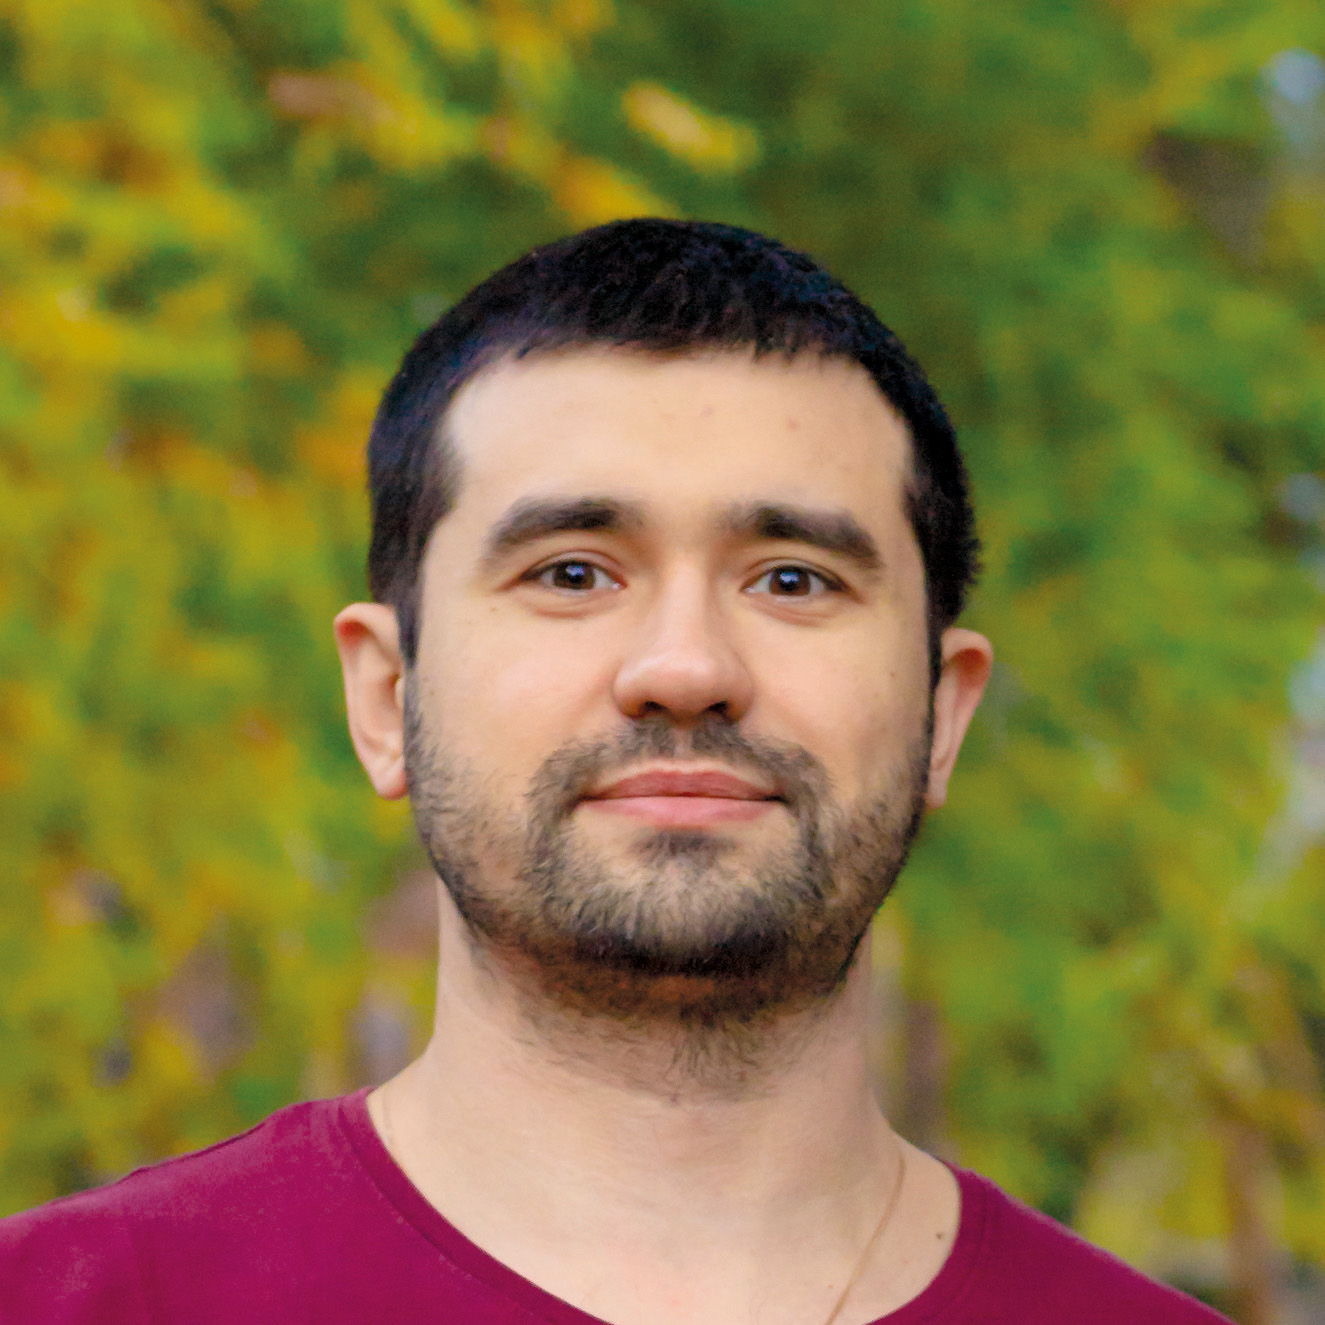
\includegraphics[width=2cm, height=2cm]{media/avatar_rgb.jpg}};
\end{tikzpicture}

\end{minipage}

&
  \vspace{0.25cm}
  {\Large\textbf{Об авторе}}

\end{tabular}

{\small

\noindent
Иван Гришаев~--- увлеченный программист. Последние восемь лет занимается языком
Clojure и редактором Emacs. Работает удаленно в стартапе Audience
Republic. Ведет блог о программировании и удаленной работе \SITELINK.
}

\else

\begin{tabular}{ @{}p{2.5cm} @{}p{5cm} }

\begin{minipage}{2.5cm}
\begin{tikzpicture}
\clip (0,0) circle (1cm) node {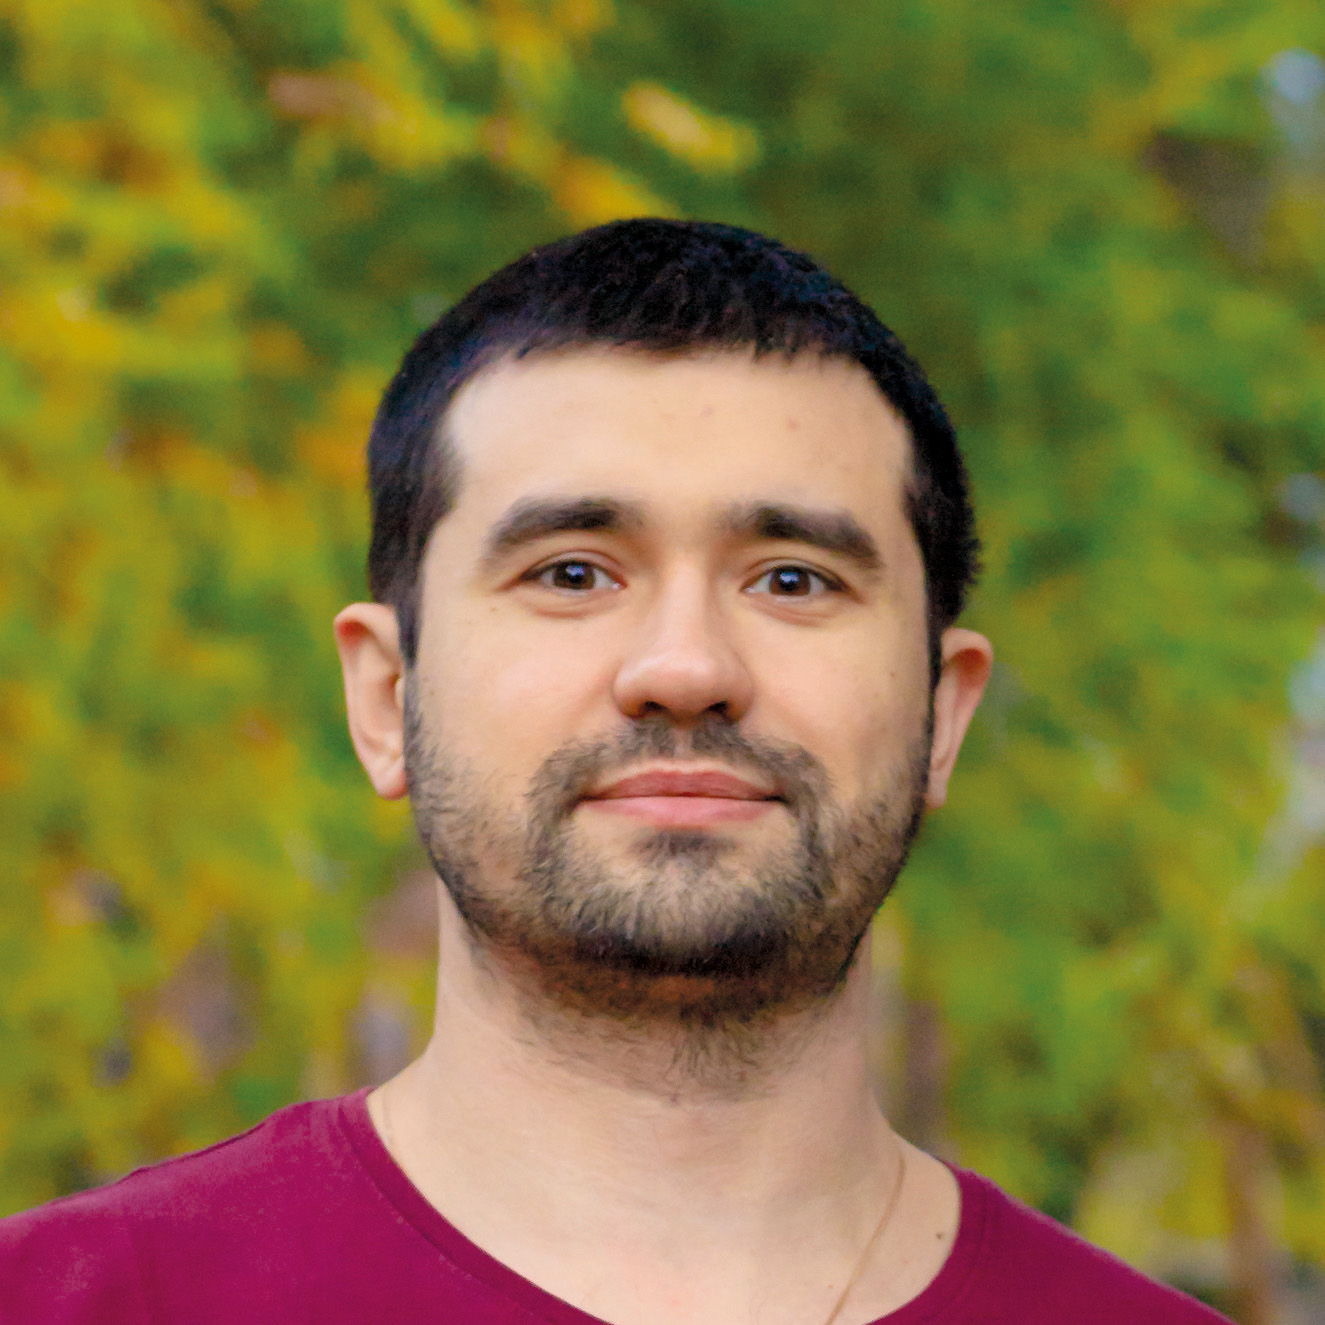
\includegraphics[width=2cm, height=2cm]{media/avatar_rgb.jpg}};
\end{tikzpicture}

\end{minipage}

&

\vspace{-1cm}

\section*{Об авторе}

{\small

Иван Гришаев~--- увлеченный программист. Последние восемь лет занимается языком
Clojure и редактором Emacs. Работает удаленно в стартапе Audience
Republic. Ведет блог о программировании и удаленной работе \SITELINK.

}

\end{tabular}
\fi

\fi

\end{document}
